\documentclass[12pt, a4paper]{article}
\usepackage{babel}
\usepackage{cleveref}
\usepackage{graphicx}

% Setter mindre marginer for å få mer plass
\usepackage[margin=2.5cm]{geometry}

% Pakke for å ha figurer side om side
\usepackage{subcaption}

% Pakke for å ha figurer ved siden av tekst
\usepackage{wrapfig}

% Kommando som gjør at bilder kan være i en mappe som heter "bilder"
\graphicspath{ {./bilder/} }

% Må ha for referanselista
\usepackage{url}

% For å tegne figurer
\usepackage{tikz}
\usetikzlibrary{calc,trees,positioning,arrows,chains,shapes.geometric,  decorations.pathreplacing,decorations.pathmorphing,shapes,  matrix,shapes.symbols}


\title{
    Project \#3\\
    \large TLC59208F Control\\
}
\author{
    Stein Lysberg
}

\begin{document}
\tikzstyle{block} = [rectangle, draw, text width=8em, text centered, rounded      corners, minimum height=1.6em]


    \maketitle
    \tableofcontents
    \thispagestyle{empty}
    \addtocounter{page}{-1}
    \clearpage

    \section{Introduction}

        This report is the third in a series of five, and looks at the use of a Texas Instruments TLC59208F LED driver (TLC), for use with a Nordic Semiconductor nRF52DK (nRF52), 
        to make a plastic scanner. The TLC will be used to control six LEDs, and make them blink in a sequence. In later assignments a photodiode
        will be used to read how the light from these LEDs reflects off some object, to try to determine what type of plastic it contains. This report considers configuration,
        control functions, and testing. It also compares this projects implementation to that of the Arduino code the project is based on.

    \subsection{Configuration}

        The TLC has a range of configuration options, so before it can be used it need to be configured for this specific project.
        This is done by writing to its control registers. In order to
        write to these registers, communication between the TLC and the nRF52 needs to be established, which is 
        done using I$^2$C. The Zephyr RTOS has many functions for I$^2$C communication, and to access
        these, the TLC must be added to the devicetree.

        \begin{figure}[h]
                \vspace{10pt}
                \begin{subfigure}[t]{\textwidth}
                    \centering
                    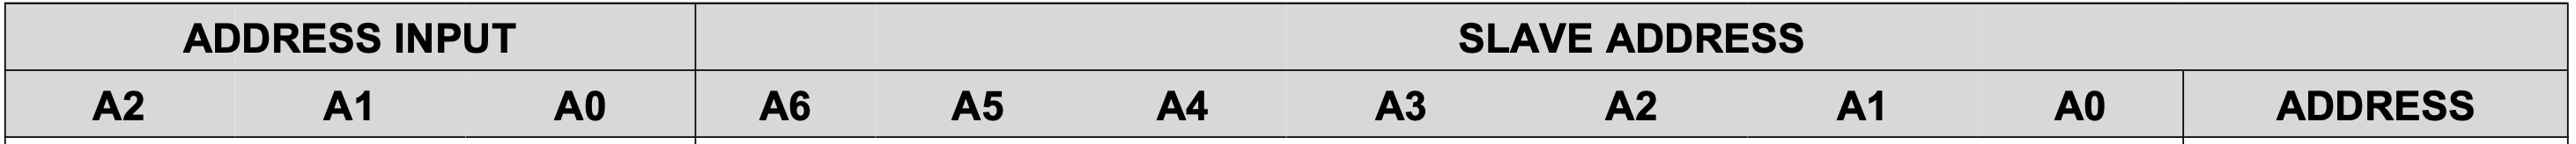
\includegraphics[width=\textwidth]{tlc_address_1.png}
                \end{subfigure}
                \begin{subfigure}[t]{\textwidth}
                    \centering
                    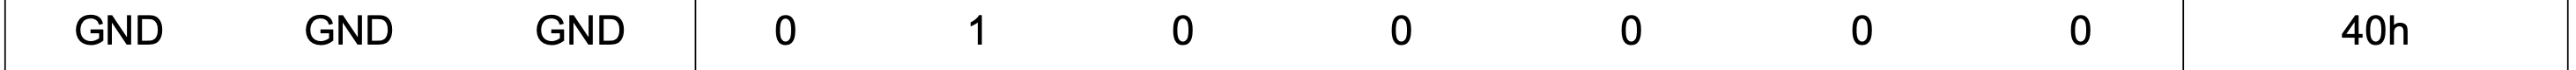
\includegraphics[width=\textwidth]{tlc_address_2.png}
                \end{subfigure}
                \caption{Address table for the TLC (cropped) \cite{tlc}.}
                \label{fig:addresstable}
            \end{figure}

        \subsubsection{Finding the I$^2$C address}

            \begin{wrapfigure}[13]{r}{0.5\textwidth}
            \centering
            \vspace{-40pt}
            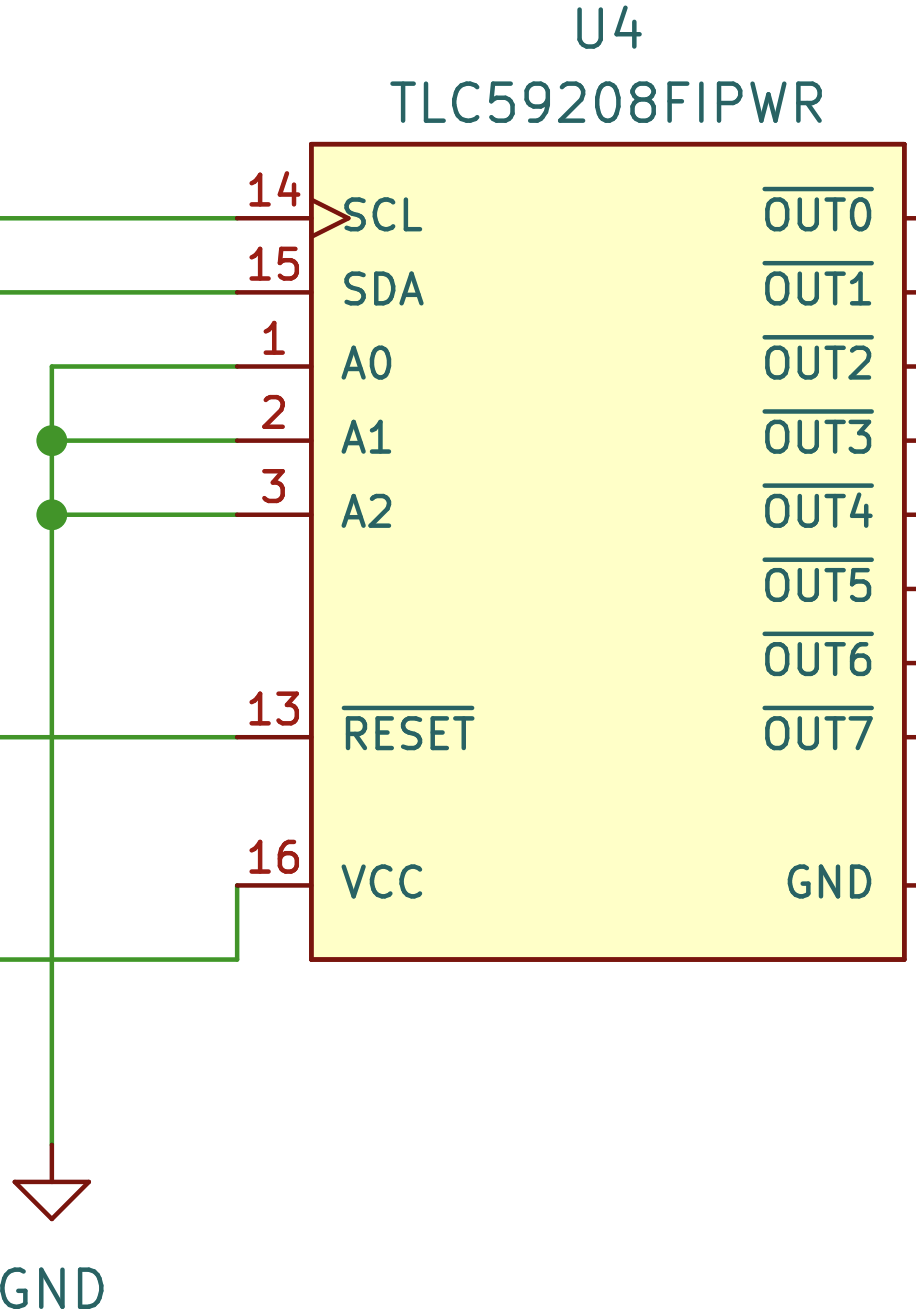
\includegraphics[width=0.3\textwidth]{gnd.png}
            \caption{Adress inputs on the TLC \cite{DB23}.}
            \label{fig:tlc_gnd}
            \end{wrapfigure}

            To communicate with the TLC, the devices I$^2$C-address must be acquired. The method for determining and finding the address is
            found in the user manual \cite{tlc}. As \cref{fig:addresstable}
            shows, when all address inputs of the TLC are grounded (as they are in the plastic scanner, shown in \cref{fig:tlc_gnd}),
            the I$^2$C-address is 0b00100000, or 0x20, as shown by bits A6-A0.

            
        \subsubsection{Devicetree}

            When the I$^2$C-address for the TLC is known, it can be added to the devicetree. 
            The Nordic Semiconductor development interface, nRF Connect, already has a library to include a Texas Instruments
            TLC59108, a device similar to the one used in this project. In the hopes that it was similar enough, it was added to the devietree using the
            graphical user interface in nRF Connect as shown in \cref{fig:devicetree}. All this library does is
            include the TLC as a generic I$^2$C-device, which is what would have been done anyways.

            \begin{figure}[hbt!]
                \centering
                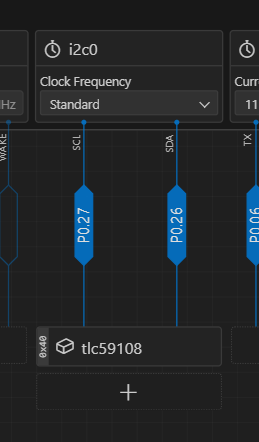
\includegraphics[width=0.4\textwidth]{devicetree}
                \caption{Adding TLC to devicetree using the graphical user interface.}
                \label{fig:devicetree}
            \end{figure}



        \subsubsection{Registers}

            When the devicetree and I$^2$C is ready, the control registers can be written to. This project uses the
            default settings of the TLC for all values except one. Upon power up, the default setting for the TLC is to enter
            \textit{low power mode}. In this application there is always one LED on, and there is no need to save power, therefore the device is instead
            configured to be in normal mode.
        
    \subsection{Control}

        Once the configuration is done, the device is ready to be used. In this project, the TLC used to loop through
        six LED, turning them on and off one at a time. \Cref{fig:ledout} shows how the registers should be written to (for the second of the
        2 LEDOUT registers, but it is the same for the first). The 8 bits in the register are divided into four groups of 2, where each group
        represents one LED. To turn a LED fully on, the value 0b01 must be written to the appropriate group.

        \begin{figure}[hbt!]
                \centering
                \fbox{
                    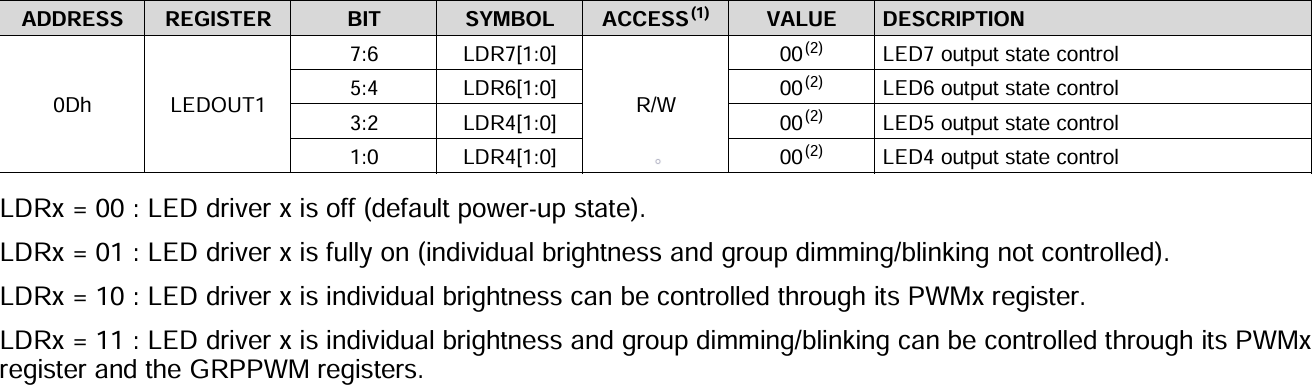
\includegraphics[width=0.9\textwidth]{ledout}
                }
                \caption{LEDOUT1 register \cite{tlc}.}
                \label{fig:ledout}
            \end{figure}

        
    \subsection{Testing}
        \begin{wrapfigure}[5]{r}{0.5\textwidth}
            \centering
            \vspace{-30pt}
            \begin{tikzpicture}
                [node distance=0.8cm,
                start chain=going below,]
                \node (n1) at (0,0) [block]  {LED on};
                \node (n2) [block, below of=n1] {Delay};
                \node (n3) [block, below of=n2] {LED off};
                \node (n4) [block, below of=n3] {Go to next};

                % Connectors
                \draw [->] (n1) -- (n2);
                \draw [->] (n2) -- (n3);
                \draw [->] (n3) -- (n4);
                \draw [->] (n4.west) -| ++(-0.4,0) |- (n1.west);
            \end{tikzpicture}
            \caption{Test cycle.}
            \label{fig:testcycle}
        \end{wrapfigure}


        \Cref{fig:testcycle} shows the flow of the loop implemented to test the TLC, after the configuration is done.
        To confirm that the implementation has been successful, it is sufficient
        to see that the LEDs go on and off in a circle. However, the LEDs emit wavelengths between 940nm and 1550nm, which
        are invisible to the human eye. In order to confirm that the LEDs actually turn on, they can be observed by using a camera
        that doesn't filter these frequencies. Alternatively, voltages across the LEDs can be measured. This will not confirm that they light
        up, only that they get voltage.

\section{Discussion}

    \begin{wrapfigure}[5]{r}{0.5\textwidth}
            \centering
            \vspace{-40pt}
            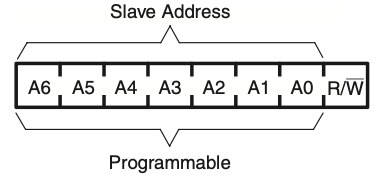
\includegraphics[width=0.4\textwidth]{tlc_address_scheme.png}
            \caption{Adress scheme of the TLC \cite{tlc}.}
            \label{fig:address_scheme}
        \end{wrapfigure}

    In this section we will discuss an issue with ambiguity of the I$^2$C-address for the TLC, point out some
    things the Arduino-code does inefficiently, and address an issue with LED visibility encountered during testing.

    \subsection{I$^2$C-address}

        \begin{wrapfigure}[18]{r}{0.34\textwidth}
            \centering
            \vspace{-30pt}
            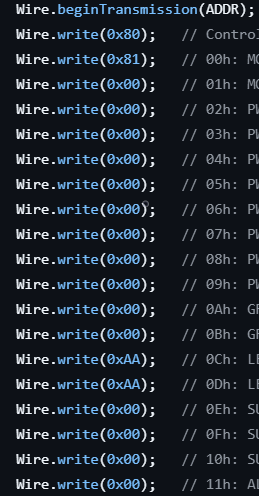
\includegraphics[width=0.28\textwidth]{configsnip.png}
            \caption{Register values in the Arduino code \cite{arduinocode}.}
            \label{fig:configsnip}
        \end{wrapfigure}

    Some time was spent troubleshooting due to having the wrong I$^2$C-address. \Cref{fig:addresstable} shows the address to be
    0x20, but to the right of this figure it says "Address: 40h". This was interpreted to mean that the address should be 0x40, which is wrong.
    The ambiguity is with wether or not the R/W-bit shown in \cref{fig:address_scheme} is part of the address or not. This bit is part of
    the \textit{register which holds the address}, but is not a part of the address itself. This means that when the register has the value 0x40,
    the address is 0x20.
            

    \subsection{Control registers}


    When the TLC is configured for this application, only one register value is changed, and the default settings are used for the rest.
    The Arduino code does this differently to this project. It utilizes the \textit{auto-increment} functionality of the TLC, which lets it receive an number of values in a row,
    and the values are sent to register addresses in ascending order \cite{tlc}. Using this, nearly \textit{all} registers are written to,
    as shown in \cref{fig:configsnip} \cite{arduinocode}. Most of the values written here are 0x00, which is mostly default values. A cleaner
    solution would be to only write to the registers that need configuring. This makes the setup faster, and the code more readable. 

    \subsection{PWM vs. LEDOUT}

    Another difference between the code for this project and the Arduino code, is that the Arduino code uses pulse width modulation (PWM) to
    control the LEDs. The documentation for the TLC states that the PWM operates at 97 kHz, with a maximum duty cycle of 99,6\% \cite{tlc}. The purpose
    of PWM in the TLC is to dim the lights for applications where full brightness is undesired. In this application there is no reason to
    use the LEDs below full brightness. Using PWM also gives a small (0.4\%) chance that a LED will be dark when a scan is being done, because of the 99,6\% duty cycle. In
    this project, the LEDOUT register of the TLC is written to directly, causing LEDs to either be fully on or fully off.

    \subsection{Visibility of LEDs}
    
    As stated previously, the LEDs which are being controlled emit wavelengths invisible to the human eye, but they can be seen by using a camera
    that doesn't filter these frequencies. It shoould be noted that some cameras have more effective filters than others.
    The phone cameras which were tested all picked up D4 and D5 (940 and 1050nm). D6 and D7 (1200 and 1300nm) was detectable with some cameras
    and the light from LEDs D8 and D9 (1460 and 1550nm) has not been detected by any of the cameras that have been tested. The code has been confirmed as working by instead measuring the voltage
    across these LEDs.

    

\section{Conclusion}
    This report has discussed the implementation of a TLC59208F LED driver as part of the plastic scanner.
    The necessary steps for successful implementation has been explained, and some improvements from the Arduino code being mimicked \cite{arduinocode}
    have been pointed to. Namely, writing to the LEDOUT registers rather than using PWM for better control of the LEDs, as well as not
    writing default values to registers, for a more effective setup. An ambiguity in the I$^2$C-address, where the value of the address is
    different from the value contained in the register which holds the address, has also been clarified. Lastly, a challenge with LEDs emitting invisible
    wavelengths has been addressed.

    \clearpage
    \addcontentsline{toc}{section}{References}  
    \bibliographystyle{IEEEtran}
    \bibliography{bibliography}

\end{document}